\section{Auswertung}

Bei der Nullmessung wird ein Zeitintervall von $\increment t = 900$ gewählt und
es werden zwei Messungen durchgeführt, deren Mittelwert für weitere Berechnungen
verwendet wird:

\begin{align*}
  N\ua{1}                &= 218 \\
  N\ua{2}                &= 224 \\
  \bar{N}                &= 221 \\
  \sigma\ua{Nullmessung} &= 14.87
\end{align*}

Alle Fehler der folgenden Messungen wurden mit der Gauß´schen Fehlerfortpflanzung
errechnet und die verschiedenen Abbildungen wurden mit Python angefertigt. Dabei
wird für die Anzahl der Zerfälle $N$ ein Fehler von $\sqrt{N}$ verwendet.
Desweiteren wird bei allen Messungen eine lineare Regression in der folgenden Form
verwendet, um die Zerfallskonstante zu bestimmen:

\begin{equation}
  f(x) = -A \cdot x + B
  \label{eqn:linRegress}
\end{equation}

Bei der Formel handelt es sich um eine Anpassung an die Exponentialfunktion, sodass
sich folgende Beziehungen für die Konstanten ergeben:

\begin{align}
  A &= \lambda
  \label{eqn:LambdaA} \\
  B &= \ln{N_0}
  \label{eqn:NnullB}
\end{align}

\subsection{Halbwertszeit von Indium}

Bei der Messung von Indium wird ein Zeitintervall von $\increment t = 240 \,
\su{s}$ und ein Messzeitraum von $t\ua{ges} = 3600 \, \su{s}$ gewählt. Die
gemessenen Zerfälle sind in Tabelle \ref{tab:Indium} eingetragen und grafisch
in Abbildung \ref{fig:Indium} dargestellt.

\begin{table}
  \centering
  \caption{Gemessene Zerfälle bei Indium.}
  \label{tab:Indium}
  \begin{tabular}{c c c c c}
    \toprule $t$ in $\su{s}$ & Anz. Zerfaelle & $\sigma_N$ & $\sigma_{N,u}$ & $\sigma_{N,o}$ \\
    \midrule
    240 & 2995  & 54 & 0.02 & 0.02 \\
    720 & 2465  & 49 & 0.02 & 0.02 \\
    1200 & 2345 & 49 & 0.02 & 0.02 \\
    1680 & 2076 & 48 & 0.02 & 0.02 \\
    2160 & 1894 & 48 & 0.02 & 0.02 \\
    2640 & 1686 & 47 & 0.02 & 0.02 \\
    3120 & 1525 & 45 & 0.02 & 0.02 \\
    3600 & 1417 & 43 & 0.02 & 0.02 \\
    480  & 2485 & 43 & 0.02 & 0.02 \\
    960  & 2346 & 42 & 0.02 & 0.02 \\
    1440 & 2268 & 40 & 0.03 & 0.02 \\
    1920 & 1943 & 39 & 0.03 & 0.03 \\
    2400 & 1827 & 38 & 0.03 & 0.03 \\
    2880 & 1555 & 38 & 0.03 & 0.03 \\
    3360 & 1512 & 37 & 0.03 & 0.03 \\
    \bottomrule
  \end{tabular}
\end{table}

\begin{figure}
  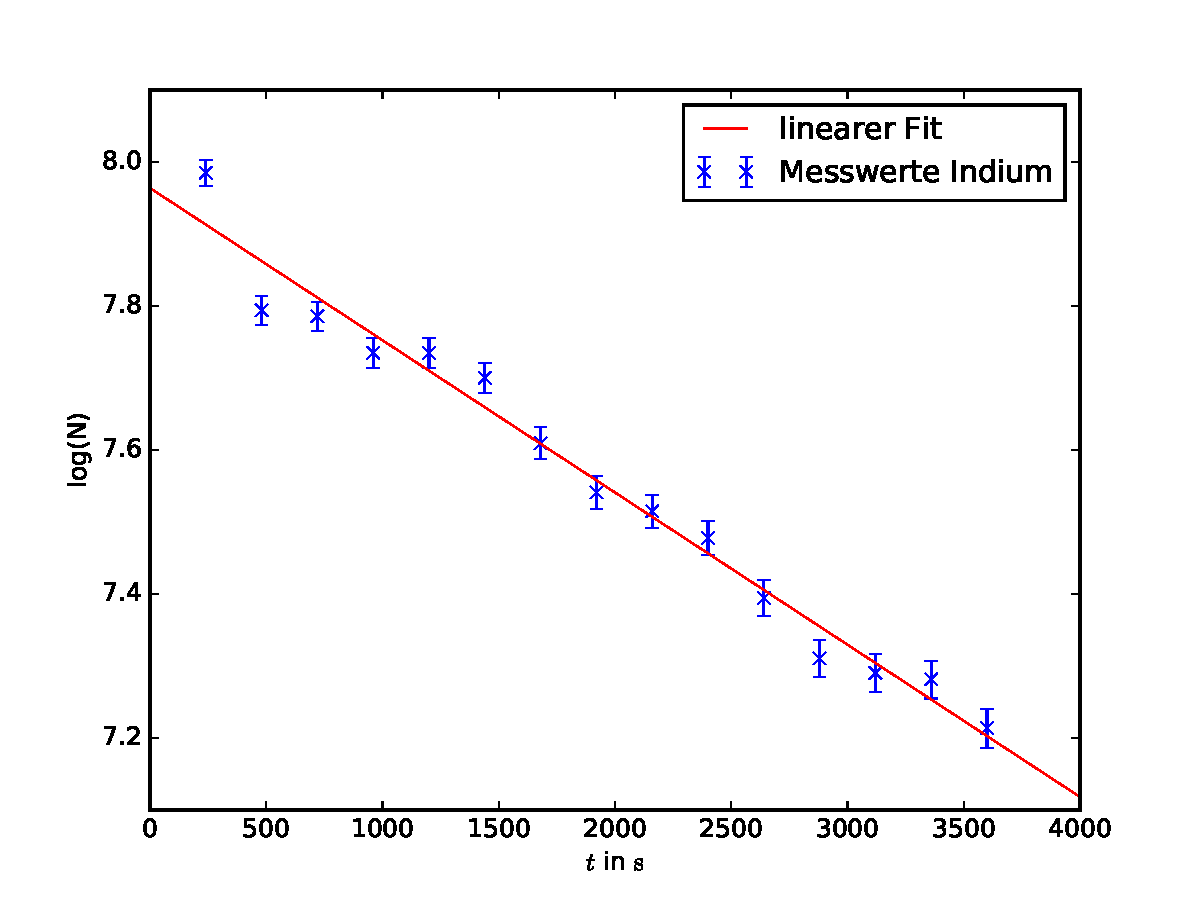
\includegraphics[width = \textwidth]{Indium_log.pdf}
  \caption{logarithmische Darstellung der gemessenen Zerfälle (N) bei Indium.}
  \label{fig:Indium}
\end{figure}

Mithilfe einer linearen Regression der Form \eqref{eqn:linRegress} und den Beziehungen
gemäß Formel \eqref{eqn:LambdaA} und \eqref{eqn:NnullB} werden dabei die Zeitkonstante
$\lambda$ und $N\ua{0,Indium}$ bestimmt:

\begin{align*}
\lambda\ua{Indium} &= A = (0.0002 \pm 9 \cdot 10^{-6}) \, \frac{1}{\su{s}}\\
N\ua{0,Indium}     &= \exp{B} = \exp{(7.96 \pm 0.02)} = (2.88 \pm 0.06) \cdot 10^{3}
\end{align*}

\begin{align}
  \label{eqn:Halbwert}
  T(\lambda) &= \frac{ln(2)}{\lambda} \\
  \label{eqn:HalbwertFehler}
  \sigma_{T} &= \frac{ln(2)}{\lambda^2} \cdot \sigma_{\lambda}
\end{align}


Mit der Formel \eqref{eqn:Halbwert} kann aus der bestimmten Zeitkonstante nun die Halbwertzeit von
Indium bestimmt werden, für die sich der folgende Wert ergibt:

\begin{equation*}
  T\ua{Indium} = (3278 \pm 141) \, \su{s}
\end{equation*}

\subsection{Halbwertszeit von Rhodium}

Bei der Messung mit $\ce{_{45}^{103}Rd}$ wird ein Zeitintervall von $\increment t = 12 \,
\su{s}$ und ein Messzeitraum von $t\ua{ges} = 720 \, \su{s}$ gewählt. Die gemessenen
Zerfälle sind in Tabelle \ref{tab:Rhodium} eingetragen sowie grafisch in Abbildung
\ref{fig:RhodiumOhne} dargestellt.

\begin{table}
  \centering
  \caption{Gemessene Zerfälle bei Rhodium.}
  \label{tab:Rhodium}
  \begin{tabular}{c c c c c c}
    \toprule $\increment t \, in \, \su{s}$ & $Anz. \, Zerfaelle$ & $\increment t \, in \, \su{s}$ & $Anz. \, Zerfaelle$
           & $\increment t \, in \, \su{s}$ & $Anz. \, Zerfaelle$ \\
    \midrule
    15 & 630 & 30 & 517 & 45 & 445 \\
    60 & 330 & 75 & 265 & 90 & 212 \\
    105 & 192 & 120 & 176 & 135 & 152 \\
    150 & 116 & 165 & 99 & 180 & 98 \\
    195 & 92 & 210 & 64 & 225 & 55 \\
    240 & 60 & 255 & 55 & 270 & 61 \\
    285 & 51 & 300 & 51 & 315 & 33 \\
    330 & 40 & 345 & 48 & 360 & 28 \\
    375 & 32 & 390 & 35 & 405 & 33 \\
    420 & 25 & 435 & 22 & 450 & 29 \\
    465 & 18 & 480 & 27 & 495 & 22 \\
    510 & 22 & 525 & 25 & 540 & 25 \\
    555 & 22 & 570 & 20 & 585 & 22 \\
    600 & 13 & 615 & 24 & 630 & 23 \\
    645 & 12 & 660 & 21 & 675 & 19 \\
    690 & 18 & 705 & 15 & 720 & 14 \\
    \bottomrule
  \end{tabular}
\end{table}

\begin{figure}
  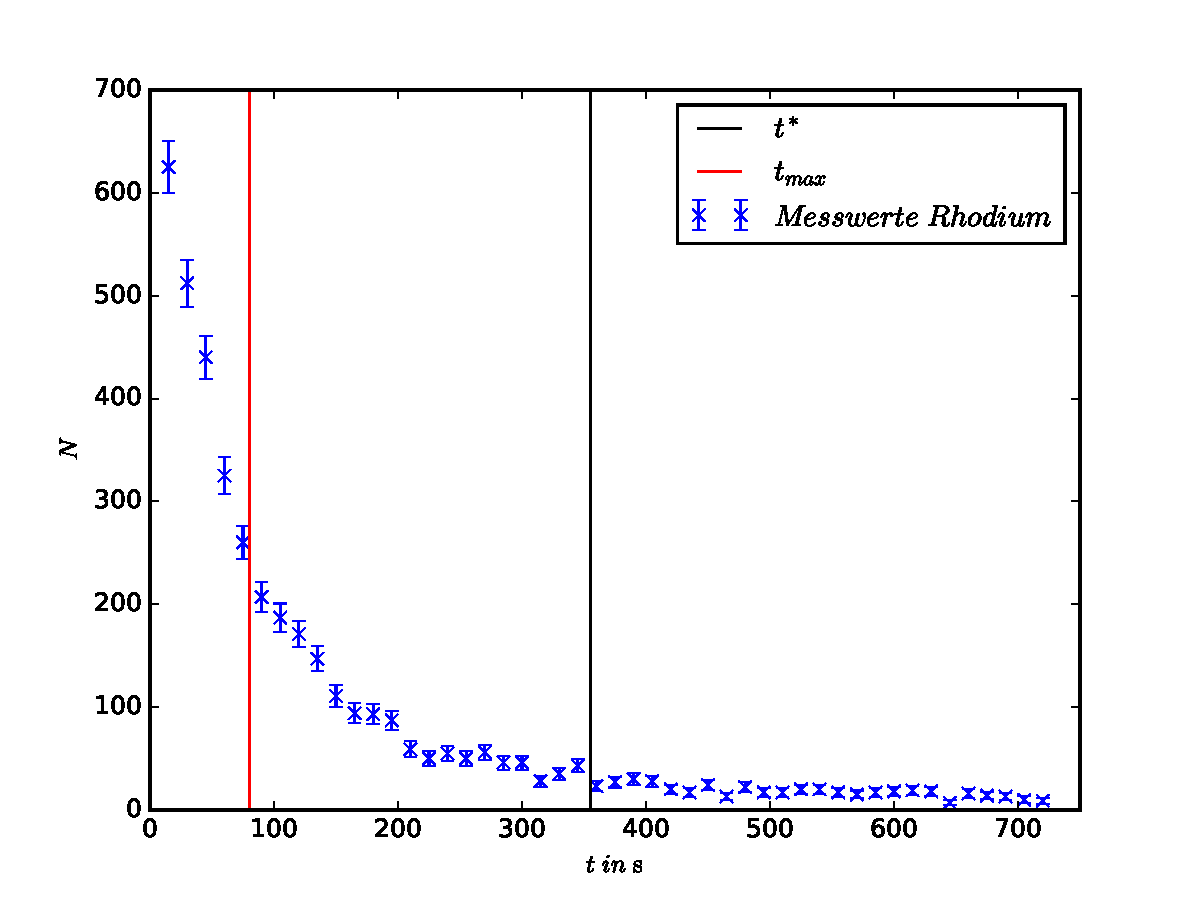
\includegraphics[width = \textwidth]{Rhodium_normal_ohne.pdf}
  \caption{Gemessene Zerfälle (N) bei Rhodium.}
  \label{fig:RhodiumOhne}
\end{figure}

Um die Halbwertzeiten der zwei verschiedenen Isotope $\ce{^{104}Rd}$ sowie $\ce{^{104i}Rd}$
zu bestimmen, die bei der Aktivierung von $\ce{_{45}^{103}Rd}$ entstehen, werden für die
Unterteilung die Messzeiten $t^{*}=355 \, \su{s}$ und $t_{\su{max}}=80 \, \su{s}$ gewählt. Zusätzlich
werden von den gemessenen Werten die von den Umgebungszerfällen erzeugten Signale
subtrahiert (siehe Tabelle \ref{tab:Rhodium104i}).


\begin{table}
  \centering
  \caption{Gemessene Werte für $\ce{^{104i}Rd}$.}
  \label{tab:Rhodium104i}
  \begin{tabular}{c c c c c}
    \toprule
    $\increment t$ in $\su{s}$ & Zerfaelle $N$ & $\sigma_N$ & $\sigma_{ln,u}$ & $\sigma_{ln,o}$ \\
    \midrule
    360 & 23 & 5 & 0.2 & 0.2 \\
    375 & 37 & 5 & 0.2 & 0.2 \\
    390 & 30 & 5 & 0.2 & 0.2 \\
    405 & 28 & 5 & 0.2 & 0.2 \\
    420 & 20 & 4 & 0.3 & 0.2 \\
    435 & 17 & 4 & 0.3 & 0.2 \\
    450 & 24 & 5 & 0.2 & 0.2 \\
    465 & 13 & 4 & 0.3 & 0.2 \\
    480 & 22 & 5 & 0.2 & 0.2 \\
    495 & 17 & 4 & 0.3 & 0.2 \\
    510 & 17 & 4 & 0.3 & 0.2 \\
    525 & 20 & 4 & 0.3 & 0.2 \\
    540 & 20 & 4 & 0.3 & 0.2 \\
    555 & 17 & 4 & 0.3 & 0.2 \\
    570 & 15 & 4 & 0.3 & 0.2 \\
    585 & 17 & 4 & 0.3 & 0.2 \\
    600 & 18 & 4 & 0.3 & 0.2 \\
    615 & 19 & 4 & 0.3 & 0.2 \\
    630 & 18 & 4 & 0.3 & 0.2 \\
    645 &  7 & 3 & 0.5 & 0.3 \\
    660 & 16 & 4 & 0.3 & 0.2 \\
    675 & 14 & 4 & 0.3 & 0.2 \\
    690 & 13 & 4 & 0.3 & 0.2 \\
    705 & 10 & 3 & 0.4 & 0.3 \\
    720 &  9 & 3 & 0.4 & 0.3 \\
    \bottomrule
  \end{tabular}
\end{table}

\begin{figure}
  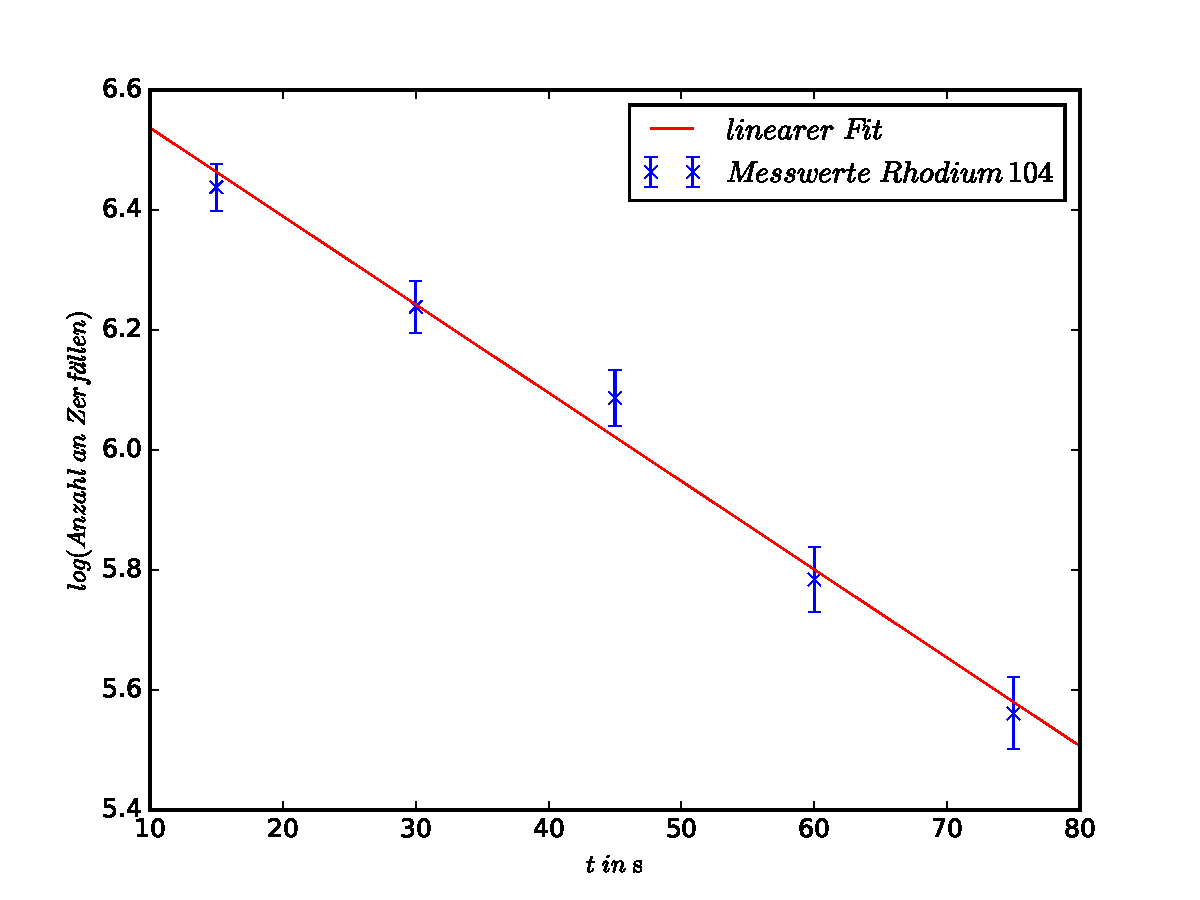
\includegraphics[width = \textwidth]{Rhodium_links_log.pdf}
  \caption{logarithmische Darstellung der gemessene Zerfälle (N) für $t > t^{*}$ bei $\su{Rh}^{104i}$.}
  \label{fig:Rh104i}
\end{figure}

Mithilfe einer linearen Regression gemäß Formel \eqref{eqn:linRegress} können
dann mithilfe der Werte für $t > t^{*}$ (Abbildung \ref{fig:Rh104i}) zuerst die beiden Parameter
für $\ce{^{104i}Rd}$ bestimmt werden:

\begin{align*}
  A                  &= \lambda\ua{Rhodium\,104i} = (0.0023 \pm 0.0004) \, \frac{1}{\su{s}}\\
  B                  &= N\ua{0,Rhodium\,104i}     = (4.1 \pm 0.2) \\
\end{align*}


Mit den Werten und Formel \eqref{eqn:Halbwert} ergibt sich für die Halbwertszeit
von $\su{Rh}^{104i}$ folgender Wert:

\begin{equation*}
  T\ua{Rhodium\,104i} = (297 \pm 54) \, \su{s}
\end{equation*}

\begin{table}
  \centering
  \caption{Gemessene Werte für ${104}^Rd$.}
  \label{tab:Rhodium104}
  \begin{tabular}{c c c c c}
    \toprule
    $\increment t$ in $\su{s}$ & Zerfaelle $N$ & $\sigma_N$ & $\sigma_{ln,u}$ & $\sigma_{ln,o}$ \\
    \midrule
    15 & 566 & 25 & 0.05 & 0.04 \\
    30 & 455 & 23 & 0.05 & 0.05 \\
    45 & 385 & 21 & 0.05 & 0.05 \\
    60 & 272 & 18 & 0.07 & 0.07 \\
    75 & 209 & 16 & 0.08 & 0.07 \\
    \bottomrule
  \end{tabular}
\end{table}

Mithilfe der selben Vorgehensweise kann aus allen Werten für $t < t_{max}$ (Abbildung
\ref{fig:Rh104}, Tabelle \ref{tab:Rhodium104}) auch die Halbwertszeit für $\ce{^{104}Rd}$
berechnet werden. Dafür
wird vorher mithilfe der berechneten Parameter von $\ce{^{104i}Rd}$ der Anteil an Zerfällen
des langlebigen Zerfalls subtrahiert,
sodass sich folgende Parameter ergeben:

\begin{align*}
  \lambda\ua{Rhodium\,104} &= A = (0.0167 \pm 0.0011) \, \frac{1}{\su{s}}\\
  N\ua{0,Rhodium\,104}     &= \exp{B} = \exp{(6.68 \pm 0.05)} = (7.5 \pm 0.4) \cdot 10^{2}
  T\ua{Rhodium\,104} &= (41 \pm 3) \, \su{s}
\end{align*}

\begin{figure}
  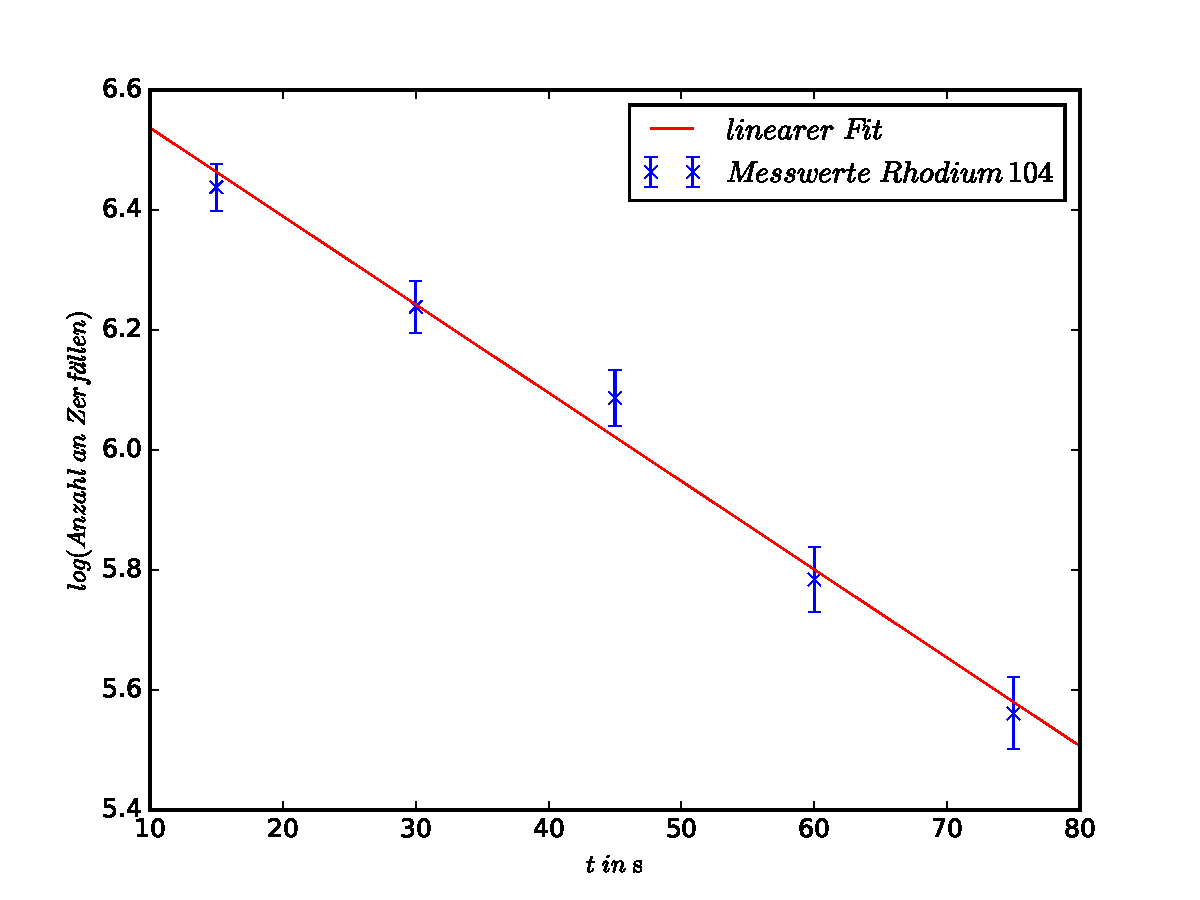
\includegraphics[width = \textwidth]{Rhodium_links_log.pdf}
  \caption{logarithmische Darstellung der gemessene Zerfälle (N) für $t < t_{max}$ bei $\su{Rh}^{104}$.}
  \label{fig:Rh104}
\end{figure}


Mit den bestimmten Parametern für $\ce{^{104}Rd}$ und $\ce{^{104i}Rd}$ kann nun
auch eine Summenkurve gezeichnet werden (Abbildung \ref{fig:Summe}).

\begin{figure}
  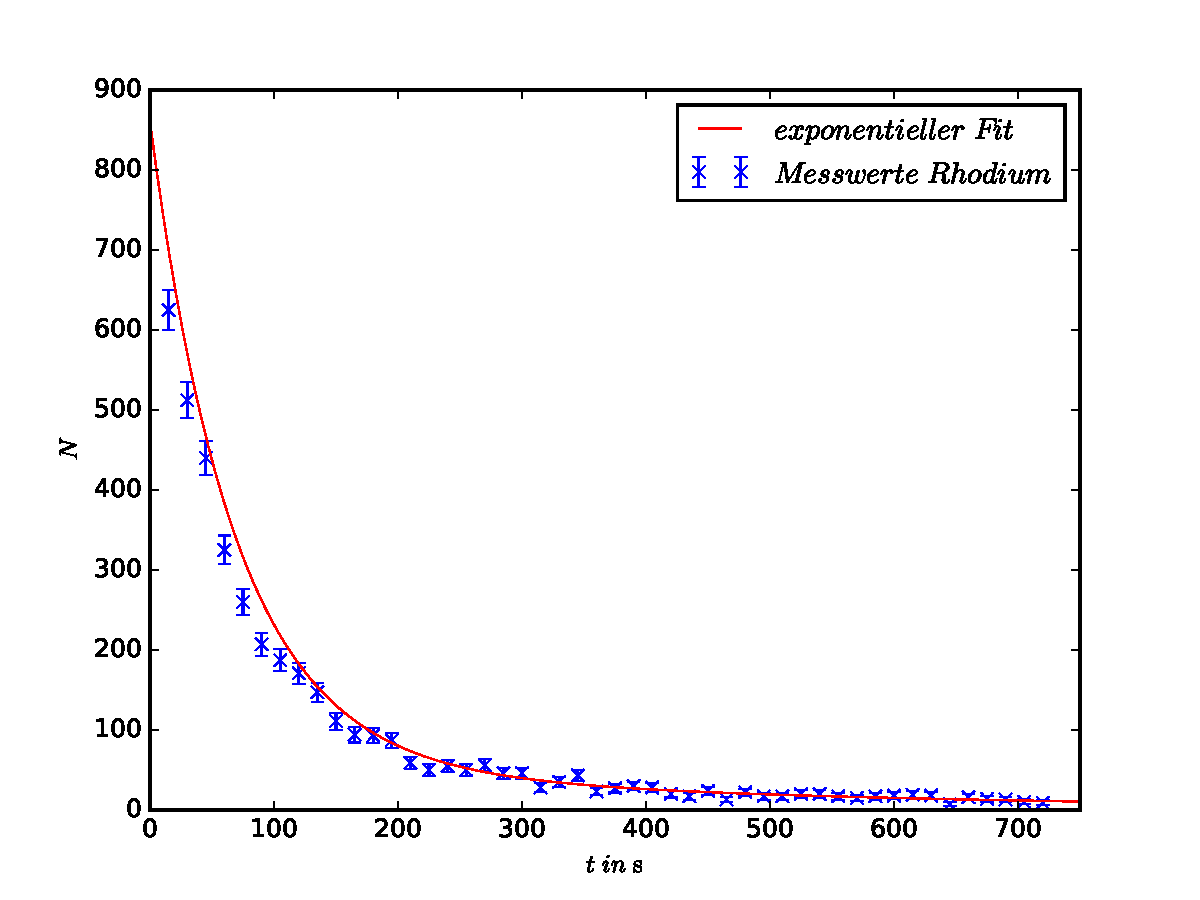
\includegraphics[width = \textwidth]{Rhodium_normal}
  \caption{Summenkurve für den Zerfall von $\ce{_{45}^{103}Rd}$.}
  \label{fig:Summe}
\end{figure}

\newpage

\section{Diskussion}

Wenn die berechneten Halbwertszeiten für $\ce{_{45}^{103}Rd}$ und $\su{In}_{49}^{115}$
mit den Literaturwerten verglichen werden, ist eine leichte Abweichung zu erkennen.
Bei allen drei bestimmten Halbwertszeiten liegt der Literaturwert im Fehlerintervall
des jeweiligen experimentell bestimmten Wert (siehe Tabelle \ref{tab:vergleich}).

\begin{table}
  \centering
  \caption{Halbwertszeiten der verschiedenen Isotope \cite{Page01}.}
  \label{tab:vergleich}
  \begin{tabular}{c c c}
    \toprule
    Isotop & $T_{exp} \, in \, \su{s}$ & $T_{Lit} \, in \, \su{s}$ \\
    \midrule
    $\su{In}_{49}^{115}$ & $3278 \, \pm \, 141$ & $3269$ \\
    $\su{Rh}^{104}$      & $41 \, \pm \, 3$     & $42.3$ \\
    $\su{Rh}^{104i}$     & $297 \, \pm \, 54$   & $274$  \\
    \bottomrule
  \end{tabular}
\end{table}

Zusammen mit dieser Erkenntnis und den verschiedenen Abbildungen lässt sich darauf
schließen, dass die auftretenden Abweichungen lediglich durch statistische Fehler
hervorgerufen werden.

Fehlerquellen können hierbei vor allem der Nulleffekt und das Geiger-Müller-Zählrohr
sein, da die von der Umgebung abgegebene Radioaktivität im Laufe des Experimentes
schwankt und nicht anhand einer vorher ausgeführten Nullmessung komplett
eliminiert werden kann.
